\documentclass[12pt]{article}
\usepackage{amsthm,amssymb,amsfonts,amsmath,amstext,systeme,adjustbox}
\usepackage{graphicx,float,wrapfig}
\usepackage{tabularx,enumitem}
\marginparwidth 0pt
\oddsidemargin -1.2 truecm
\evensidemargin  0pt 
\marginparsep 0pt
\topmargin -2.2truecm
\linespread{1}
\textheight 25.8 truecm
\textwidth 18.5 truecm
\newenvironment{remark}{\noindent{\bf Remark }}{\vspace{0mm}}
\newenvironment{remarks}{\noindent{\bf Remarks }}{\vspace{0mm}}
\newenvironment{question}{\noindent{\bf Question }}{\vspace{0mm}}
\newenvironment{questions}{\noindent{\bf Questions }}{\vspace{0mm}}
\newenvironment{note}{\noindent{\bf Note }}{\vspace{0mm}}
\newenvironment{summary}{\noindent{\bf Summary }}{\vspace{0mm}}
\newenvironment{back}{\noindent{\bf Background}}{\vspace{0mm}}
\newenvironment{conclude}{\noindent{\bf Conclusion}}{\vspace{0mm}}
\newenvironment{concludes}{\noindent{\bf Conclusions}}{\vspace{0mm}}
\newenvironment{dill}{\noindent{\bf Description of Dill's model}}{\vspace{0mm}}
\newenvironment{maths}{\noindent{\bf Mathematics needed}}{\vspace{0mm}}
\newenvironment{inst}{\noindent{\bf Instructions}}{\vspace{0mm}}
\newenvironment{notes}{\noindent{\bf Notes }}{\vspace{0mm}}
\newenvironment{theorem}{\noindent{\bf Theorem }}{\vspace{0mm}}
\newenvironment{example}{\noindent{\bf Example }}{\vspace{0mm}}
\newenvironment{examples}{\noindent{\bf Examples }}{\vspace{0mm}}
\newenvironment{topics}{\noindent{\bf Topics}}{\vspace{0mm}}
\newenvironment{outcomes}{\noindent{\bf Expected Learning Outcomes}}{\vspace{0mm}}
\newenvironment{lemma}{\noindent{\bf Lemma }}{\vspace{0mm}}
\newenvironment{solution}{\noindent{\it Solution}}{\vspace{2mm}}
\newcommand{\ds}{\displaystyle}
\newcommand{\un}{\underline}
\newcommand{\bs}{\boldsymbol}

\begin{document}

\baselineskip 18 pt
\begin{center}
	{\large \bf HKDSE MATH Core Sample Paper II}\\
	\vspace{2 mm}
\end{center}
\vspace{0.05cm}

\begin{enumerate}
	\item \textbf{HKDSE MATH Core Sample Paper II Q1}\\
	$(3a)^2 \cdot a^3 = $
	\begin{enumerate}
		\item[A.] $3a^5$.
		\item[B.] $6a^6$.
		\item[C.] $9a^5$.
		\item[D.] $9a^6$.
	\end{enumerate}

	\item \textbf{HKDSE MATH Core Sample Paper II Q2}\\
	If $5 - 3m = 2n$, then $m =$
	\begin{enumerate}
		\item[A.] $n$.
		\item[B.] $\dfrac{2n - 5}{3}$.
		\item[C.] $\dfrac{-2n + 5}{3}$.
		\item[D.] $\dfrac{-2n + 15}{3}$.
	\end{enumerate}

	\item \textbf{HKDSE MATH Core Sample Paper II Q3}\\
	$a^2 - b^2 + 2b - 1 =$
	\begin{enumerate}
		\item[A.] $(a - b - 1)(a + b - 1)$
		\item[B.] $(a - b - 1)(a + b + 1)$
		\item[C.] $(a - b + 1)(a + b - 1)$
		\item[D.] $(a - b + 1)(a - b - 1)$
	\end{enumerate}

	\item \textbf{HKDSE MATH Core Sample Paper II Q4}\\
	Let $p$ and $q$ be constants. If $x^2 + p(x + 5) + q \equiv (x - 2)(x + 5)$, then $q = $
	\begin{enumerate}
		\item[A.] $-25$.
		\item[B.] $-10$.
		\item[C.] $3$.
		\item[D.] $5$.
	\end{enumerate}

	\item \textbf{HKDSE MATH Core Sample Paper II Q5}\\
	Let $f(x) = x^3 + 2x^2 - 7x + 3$. When $f(x)$ is divided by $x + 2$, the remainder is 
	\begin{enumerate}
		\item[A.] 3.
		\item[B.] 5.
		\item[C.] 17.
		\item[D.] 33.
	\end{enumerate}

	\item \textbf{HKDSE MATH Core Sample Paper II Q6}\\
	Let $a$ be a constant. Solve tne equation $(x - a)(x - a - 1) = (x - a)$.
	\begin{enumerate}
		\item[A.] $x = a + 1$
		\item[B.] $x = a + 2$
		\item[C.] $x = a$ or $x = a + 1$
		\item[D.] $x = a$ or $x = a + 2$
	\end{enumerate}

	\item \textbf{HKDSE MATH Core Sample Paper II Q7}\\
	Find the range of values of $k$ such that the quadratic equation $x^2 - 6x = 2 - k$ has no real roots.
	\begin{enumerate}
		\item[A.] $k < -7$
		\item[B.] $k > -7$
		\item[C.] $k < 11$
		\item[D.] $k > 11$
	\end{enumerate}

	\item \textbf{HKDSE MATH Core Sample Paper II Q8}\\
	In the figure, the quadratic graph of $y = f(x)$ intersects the straight line $L$ at $A(1 , k)$ and $B(7 , k)$. Which of the following are true?
	\begin{enumerate}
		\item[I.] The solution of the inequality $f(x) > k$ is $x < 1$ or $x > 7$.
		\item[II.] The roots of the equation $f(x) = k$ are 1 and 7.
		\item[III.] The equation of the axis of symmetry of the quadratic graph of $y = f(x)$ is $x = 3$.
		\item[]
			\begin{minipage}[u]{.39\textwidth}
				\begin{enumerate}[label=(\Alph*), itemsep=0pt]
					\item[A.] I and II only
					\item[B.] I and III only
					\item[C.] II and III only
					\item[D.] I, II and III
				\end{enumerate}
			\end{minipage}
			\begin{minipage}[u]{.5\textwidth}
				\centering
				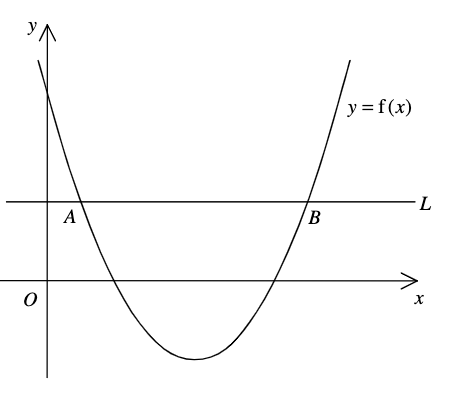
\includegraphics[scale=0.8]{SPFigure2.8.png}
			\end{minipage}
	\end{enumerate}
		
	\item \textbf{HKDSE MATH Core Sample Paper II Q9}\\
	The solution of $5 - 2x < 3$ and $4x + 8 > 0$ is 
	\begin{enumerate}
		\item[A.] $x > -2$.
		\item[B.] $x > -1$.
		\item[C.] $x > 1$.
		\item[D.] $-2 < x < 1$.
	\end{enumerate}

	\item \textbf{HKDSE MATH Core Sample Paper II Q10}\\
	Mary sold two bags for \$240 each. She gained 20\% on one and lost 20\% on the other. After the two transactions, Mary
	\begin{enumerate}
		\item[A.] lost \$20.
		\item[B.] gained \$10.
		\item[C.] gained \$60.
		\item[D.] had no gain and no loss.
	\end{enumerate}

	\item \textbf{HKDSE MATH Core Sample Paper II Q11}\\
	Let $a_n$ be the $n$th term of a sequence. If $a_1 = 4$, $a_2 = 5$ and $a_{n + 2} = a_n + a_{n + 1}$ for any positive integer $n$, then $a_{10} = $
	\begin{enumerate}
		\item[A.] 13.
		\item[B.] 157.
		\item[C.] 254.
		\item[D.] 411.
	\end{enumerate}

	\item \textbf{HKDSE MATH Core Sample Paper II Q12}\\
	If the length and the width of a rectangle are increased by 20\% and $x\%$ respectively so that its area is increased by 50\%, then $x = $
	\begin{enumerate}
		\item[A.] 20.
		\item[B.] 25.
		\item[C.] 30.
		\item[D.] 35.
	\end{enumerate}

	\item \textbf{HKDSE MATH Core Sample Paper II Q13}\\
	If $x$, $y$ and $z$ are non-zero numbers such that $2x = 3y$ and $x = 2z$, then $(x + z) : (x + y) = $
	\begin{enumerate}
		\item[A.] 3 : 5.
		\item[B.] 6 : 7.
		\item[C.] 9 : 7.
		\item[D.] 9 : 10.
	\end{enumerate}

	\item \textbf{HKDSE MATH Core Sample Paper II Q14}\\
	It is given that $z$ varies directly as $x$ and inversely as $y$. When $x = 3$ and $y = 4$ , $z = 18$ . When $x = 2$ and $z = 8$, $y = $
	\begin{enumerate}
		\item[A.] 1.
		\item[B.] 3.
		\item[C.] 6.
		\item[D.] 9.
	\end{enumerate}

	\item \textbf{HKDSE MATH Core Sample Paper II Q15}\\
	The lengths of the three sides of a triangle are measured as 15 cm, 24 cm and 25 cm respectively. If the three measurements are correct to the nearest cm , find the percentage error in calculating the perimeter of the triangle correct to the nearest 0.1\%.
	\begin{enumerate}
		\item[A.] 0.8\%
		\item[B.] 2.3\%
		\item[C.] 4.7\%
		\item[D.] 6.3\%
	\end{enumerate}

	\item \textbf{HKDSE MATH Core Sample Paper II Q16}\\
	In the figure, $O$ is the centre of the circle. $C$ and $D$ are points lying on the circle. $OBC$ and $BAD$ are straight lines. If $OC = 20$ cm and $OA = AB = 10$ cm, find the area of the shaded region $BCD$ correct to the nearest cm$^2$.
	\begin{figure}[h]
		\centering
		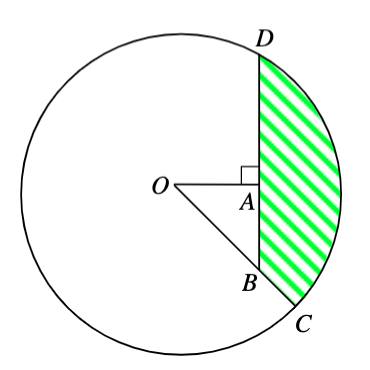
\includegraphics[width = 0.3\textwidth]{SPFigure2.16.png}	
	\end{figure}
	\begin{enumerate}
		\item[A.] 214 cm$^2$
		\item[B.] 230 cm$^2$
		\item[C.] 246 cm$^2$
		\item[D.] 270 cm$^2$
	\end{enumerate}

	\item \textbf{HKDSE MATH Core Sample Paper II Q17}\\
	The figure shows a right circular cylinder, a hemisphere and a right circular cone with equal base radii. Their curved surface areas are $a$ cm$^2$ , $b$ cm$^2$ and $c$ cm$^2$ respectively.\\
	\begin{figure}[H]
		\centering
		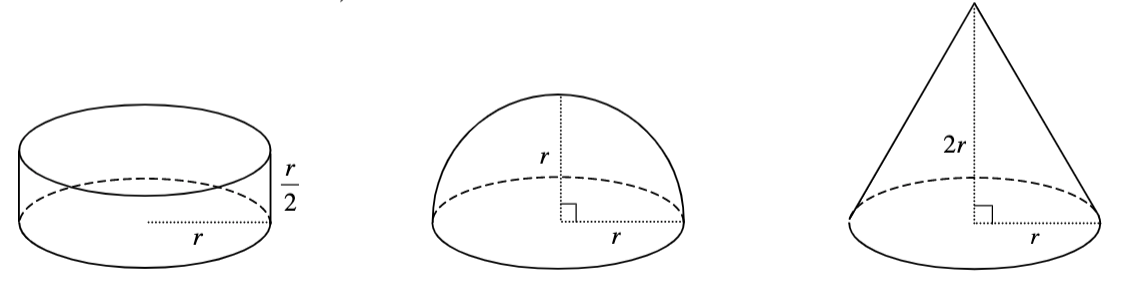
\includegraphics[width = 0.7\textwidth]{SPFigure2.17.png}	
	\end{figure}
	Which of the following is true?
	\begin{enumerate}
		\item[A.] $a < b < c$
		\item[B.] $a < c < b$
		\item[C.] $c < a < b$
		\item[D.] $c < b < a$
	\end{enumerate}

	\item \textbf{HKDSE MATH Core Sample Paper II Q18}\\
	In the figure, $ABCD$ is a parallelogram. $T$ is a point lying on $AB$ such that $DT$ is perpendicular to $AB$. It is given that $Cd = 9$ cm and $AT : TB = 1 : 2$. If the area of the parallelogram $ABCD$ is 36 cm$^2$ , then the perimeter of the parallelogram $ABCD$ is
	\begin{figure}[H]
		\centering
		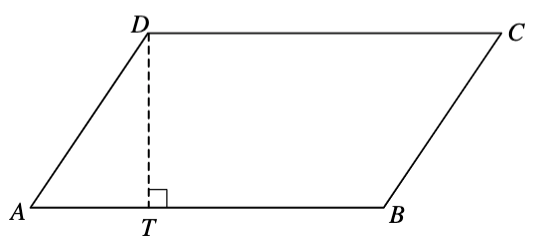
\includegraphics[width = 0.7\textwidth]{SPFigure2.18.png}	
	\end{figure}
	\begin{enumerate}
		\item[A.] 26 cm.
		\item[B.] 28 cm.
		\item[C.] 30 cm.
		\item[D.] 32 cm.
	\end{enumerate}

	\item \textbf{HKDSE MATH Core Sample Paper II Q19}\\
	$\dfrac{\sin{\theta}}{\cos{60^\circ}} + \dfrac{\cos{(270^\circ - \theta)}}{\tan{45^\circ}} = $ 
	\begin{enumerate}
		\item[A.] $\sin{\theta}$.
		\item[B.] $3\sin{\theta}$.
		\item[C.] $2\sin{\theta} - \cos{\theta}$.
		\item[D.] $2\sin{\theta} + \cos{\theta}$.
	\end{enumerate}

	\item \textbf{HKDSE MATH Core Sample Paper II Q20}\\
	In the figure, $AB = 1$ cm, $BC = CD = DE = 2$ cm and $EF = 3$ cm. Find the distance between $A$ and $F$ correct to the nearest 0.1 cm.
	\begin{figure}[H]
		\centering
		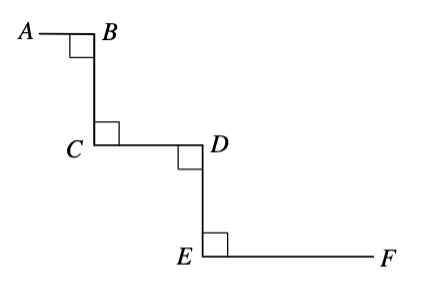
\includegraphics[width = 0.7\textwidth]{SPFigure2.20.png}	
	\end{figure}
	\begin{enumerate}
		\item[A.] 7.2 cm
		\item[B.] 7.4 cm
		\item[C.] 8.0 cm
		\item[D.] 8.1 cm
	\end{enumerate}

	\item \textbf{HKDSE MATH Core Sample Paper II Q21}\\
	In the figure, $ABCD$ is a semi-circle. If $BC = CD$, then $\angle ADC = $
	\begin{figure}[H]
		\centering
		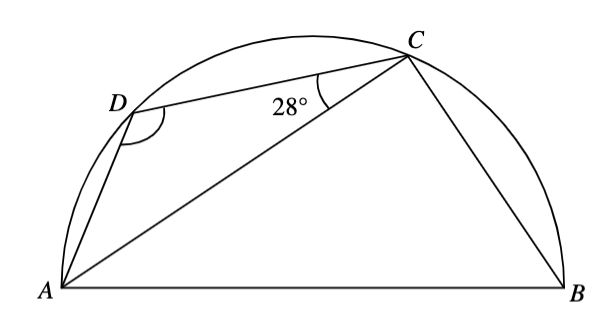
\includegraphics[width = 0.7\textwidth]{SPFigure2.21.png}	
	\end{figure}
	\begin{enumerate}
		\item[A.] 118$^\circ$.
		\item[B.] 121$^\circ$.
		\item[C.] 124$^\circ$.
		\item[D.] 126$^\circ$.
	\end{enumerate}

	\item \textbf{HKDSE MATH Core Sample Paper II Q22}\\
	In the figure, $O$ is the centre of the circle $ABCDE$. If $\angle ABE = 30^\circ$ and $\angle CDE = 105^\circ$, then $\angle AOC = $
	\begin{figure}[H]
		\centering
		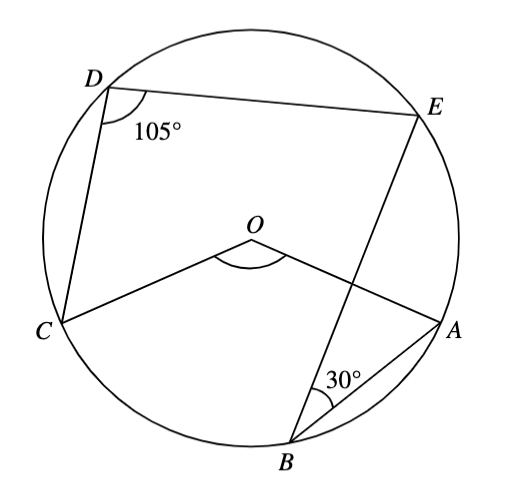
\includegraphics[width = 0.7\textwidth]{SPFigure2.22.png}	
	\end{figure}
	\begin{enumerate}
		\item[A.] 120$^\circ$.
		\item[B.] 135$^\circ$.
		\item[C.] 150$^\circ$.
		\item[D.] 165$^\circ$.
	\end{enumerate}
	
	\item \textbf{HKDSE MATH Core Sample Paper II Q23}\\
	In the figure, $ABCD$ is a parallelogram. $F$ is a point lying on $AD$. $BF$ produced and $CD$ produced meet at $E$ . If $CD : DE = 2 : 1$, then $AF : BC =$
	\begin{figure}[H]
		\centering
		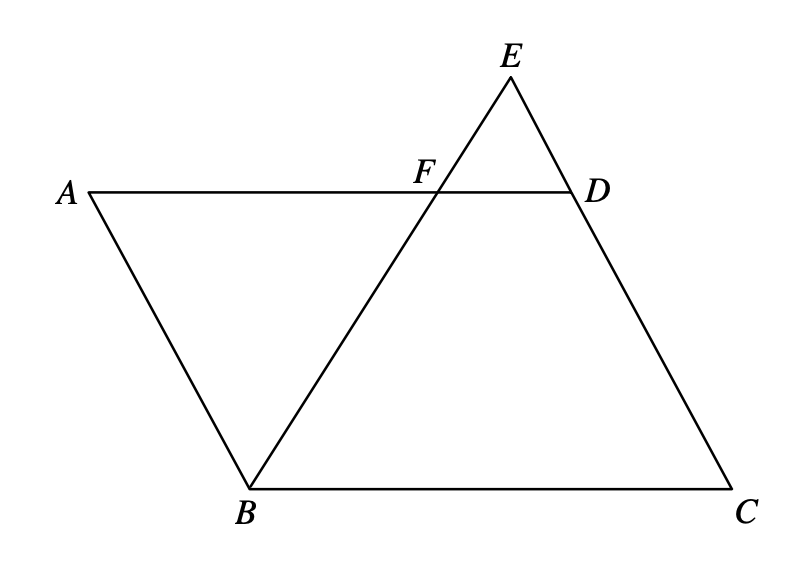
\includegraphics[width = 0.7\textwidth]{SPFigure2.23.png}	
	\end{figure}
	\begin{enumerate}
		\item[A.] $1 : 2$.
		\item[B.] $2 : 3$.
		\item[C.] $3 : 4$.
		\item[D.] $8 : 9$.
	\end{enumerate}

	\item \textbf{HKDSE MATH Core Sample Paper II Q24}\\
	In the figure, $ABC$ is a straight line. If $BD = CD$ and $AB = 10$ cm, find $BC$ corrent to the nearest cm.
	\begin{figure}[H]
		\centering
		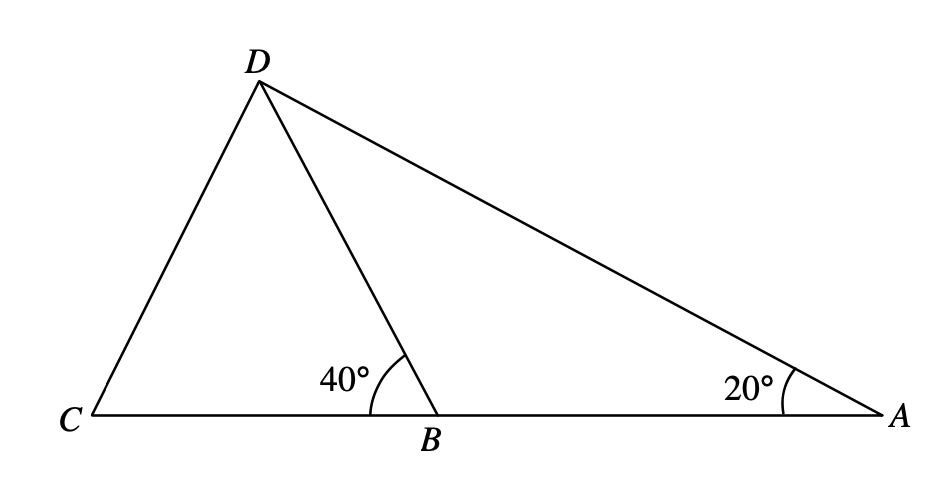
\includegraphics[width = 0.7\textwidth]{SPFigure2.24.png}	
	\end{figure}
	\begin{enumerate}
		\item[A.] 8 cm
		\item[B.] 13 cm
		\item[C.] 14 cm
		\item[D.] 15 cm
	\end{enumerate}

	\item \textbf{HKDSE MATH Core Sample Paper II Q25}\\
	In the figure, the two 6-sided polygons show
	\begin{figure}[H]
		\centering
		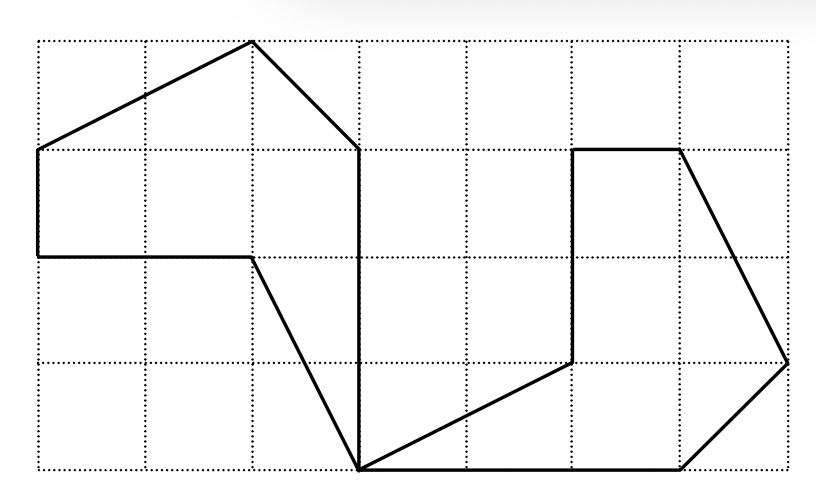
\includegraphics[width = 0.7\textwidth]{SPFigure2.25.png}	
	\end{figure}
	\begin{enumerate}
		\item[A.] a rotation transformation.
		\item[B.] a reflection transformation.
		\item[C.] a translation transformation.
		\item[D.] a dilation transformation.
	\end{enumerate}
	
	\item \textbf{HKDSE MATH Core Sample Paper II Q26}\\
	If the point $(-4, 3)$ is rotated anti-clockwise about the origin through $180^\circ$, then the coordinates of its image are
	\begin{enumerate}
		\item[A.] $(-3, -4)$.
		\item[B.] $(3, 4)$.
		\item[C.] $(-4, -3)$.
		\item[D.] $(4, -3)$.
	\end{enumerate}
	
	\item \textbf{HKDSE MATH Core Sample Paper II Q27}\\
	The box-and-whisker diagram below shows the distribution of the scores (in marks) of the students of a class in a test.
	\begin{figure}[H]
		\centering
		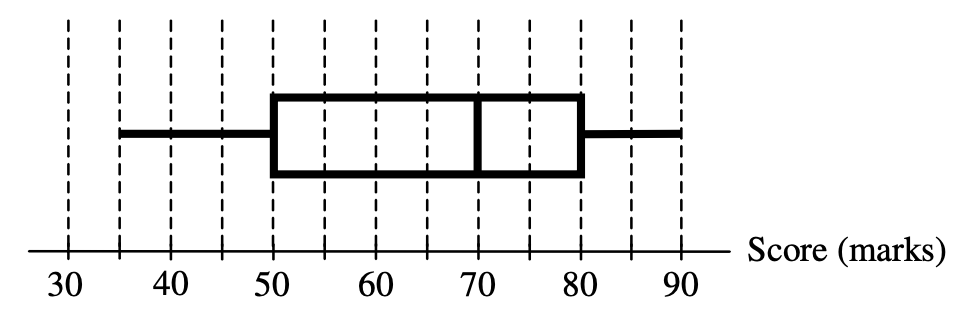
\includegraphics[width = 0.7\textwidth]{SPFigure2.27.png}	
	\end{figure}
	If the passing score of the test is 50 marks, then the passing percentage of the class is
	\begin{enumerate}
		\item[A.] 25\%.
		\item[B.] 50\%.
		\item[C.] 70\%.
		\item[D.] 75\%.
	\end{enumerate}
	
	\item \textbf{HKDSE MATH Core Sample Paper II Q28}\\
	The stem-and-leaf diagram below shows the distribution of heights (in cm) of 23 staff members in an office.
	\begin{table}[htbp]
		\centering
		\begin{tabular}{r|l@{\hspace{4 pt}}}
		    Stem (tens) & Leaf (units)\\
			\hline
			15     & 3 3 4 5 6 7 9\\    
			16     & 1 2 2 3 5 6 6 8\\    
			17     & 1 2 6 7 9\\
			18     & 2 6 7\\  
		\end{tabular}
		\label{tab:addlabel}
	\end{table}
	Find the median of the distribution.
	\begin{enumerate}
		\item[A.] 164 cm
		\item[B.] 165 cm
		\item[C.] 165.5 cm
		\item[D.] 166 cm
	\end{enumerate}
	
	\item \textbf{HKDSE MATH Core Sample Paper II Q29}\\
	$\{ a - 7 , a - 1 , a , a + 2 , a + 4 , a + 8 \}$ and $\{ a - 9 , a - 2 , a - 1 , a  +3 , a + 4 , a + 6 \}$ are two groups of numbers. Which of the following is/are true?
	\begin{enumerate}
		\item[I.] The two groups of numbers have the same mean.
		\item[II.] The two groups of numbers have the same median.
		\item[III.] The two groups of numbers have the same range.
		\item[]
		\begin{enumerate}
			\item[A.] I only
			\item[B.] II only
			\item[C.] I and III only
			\item[D.] II and III only
		\end{enumerate}
	\end{enumerate}
	
	\item \textbf{HKDSE MATH Core Sample Paper II Q30}\\
	The students' union of a school of 950 students wants to investigate the opinions of students in the school on the services provided by the tuck shop. A questionnaire is designed by the students' union and only the chairperson and vice-chairperson of the students' union are selected as a sample to fill in the questionnaire. Which of the following are the disadvantages of this sampling method?
	\begin{enumerate}
		\item[I.] The sample size is very small.
		\item[II.] Not all students in the school are selected.
		\item[III.] Not all students in the school have an equal chance of being selected.
		\item[]
		\begin{enumerate}
			\item[A.] I and II only
			\item[B.] I and III only
			\item[C.] II and III only
			\item[D.] I, II and III
		\end{enumerate}
	\end{enumerate}
	
	\item \textbf{HKDSE MATH Core Sample Paper II Q31}\\
	$\dfrac{1}{2 - x} + \dfrac{x - 1}{(x - 2)^2} = $
	\begin{enumerate}
		\item[A.] $\dfrac{-2}{(2 - x)^2}$.
		\item[B.] $\dfrac{1}{(2 - x)^2}$.
		\item[C.] $\dfrac{-2x + 3}{(2 - x)^2}$.
		\item[D.] $\dfrac{2x - 3}{(2 - x)^2}$.
	\end{enumerate}
	
	\item \textbf{HKDSE MATH Core Sample Paper II Q32}\\
	The graph in the figure shows the linear relation between $x$ and $\log_5{y}$. If $y = ab^x$, then $a =$
	\begin{figure}[H]
		\centering
		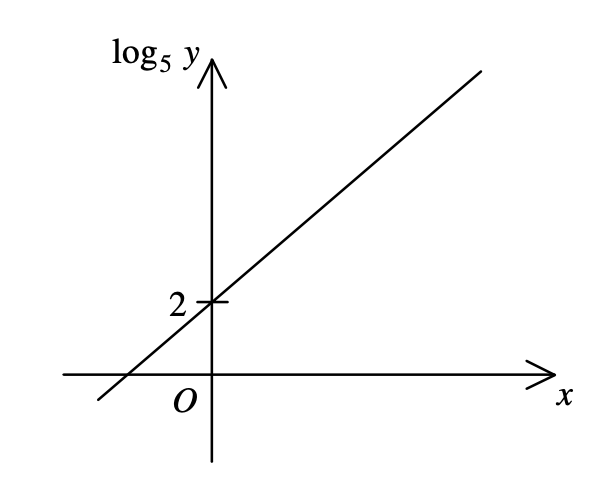
\includegraphics[width = 0.7\textwidth]{SPFigure2.32.png}	
	\end{figure}
	\begin{enumerate}
		\item[A.] 1.
		\item[B.] 2.
		\item[C.] 5.
		\item[D.] 25.
	\end{enumerate}
	
	\item \textbf{HKDSE MATH Core Sample Paper II Q33}\\
	$1010010001001_2 = $
	\begin{enumerate}
		\item[A.] $2^{12} + 2^{10} + 137$.
		\item[B.] $2^{12} + 2^{10} + 273$.
		\item[C.] $2^{13} + 2^{11} + 137$.
		\item[D.] $2^{13} + 2^{11} + 273$.
	\end{enumerate}
	
	\item \textbf{HKDSE MATH Core Sample Paper II Q34}\\
	If $k$ is a real number, then $4k - \dfrac{6 + ki}{i} = $
	\begin{enumerate}
		\item[A.] $3k + 6i$.
		\item[B.] $3k - 6i$.
		\item[C.] $5k + 6i$.
		\item[D.] $5k - 6i$.
	\end{enumerate}
	
	\item \textbf{HKDSE MATH Core Sample Paper II Q35}\\
	Which of the triangular regions in the figure may represent the solution of $\left\{
		\begin{matrix}
			0 \leq x \leq 6\\
			0 \leq y \leq 3\\
			x \leq 2y\\
		\end{matrix}\right.$?
	\begin{enumerate}
		\item[A.] $\triangle OAC$
		\item[B.] $\triangle OBD$
		\item[C.] $\triangle OCE$
		\item[D.] $\triangle ODF$
	\end{enumerate}
	
	\item \textbf{HKDSE MATH Core Sample Paper II Q36}\\
	If the 3rd term and the 6th term of an arithmetic sequence are 18 and $-6$ respectively, then 2nd term of the sequence is
	\begin{enumerate}
		\item[A.] $-8$.
		\item[B.] $10$.
		\item[C.] $26$.
		\item[D.] $34$.
	\end{enumerate}
	
	\item \textbf{HKDSE MATH Core Sample Paper II Q37}\\
	If the figure shows the graph of $y = f(x)$ and the graph of $y = g(x)$ on the same rectangular coordinate system, then
	\begin{figure}[H]
		\centering
		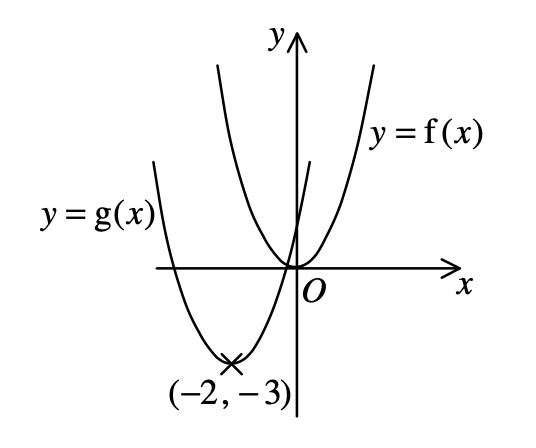
\includegraphics[width = 0.7\textwidth]{SPFigure2.37.png}	
	\end{figure}
	\begin{enumerate}
		\item[A.] $g(x) = f(x - 2) - 3$.
		\item[B.] $g(x) = f(x - 2) + 3$.
		\item[C.] $g(x) = f(x + 2) - 3$.
		\item[D.] $g(x) = f(x + 2) + 3$.
	\end{enumerate}
	
	\item \textbf{HKDSE MATH Core Sample Paper II Q38}\\
	In the figure, $y = $
	\begin{figure}[H]
		\centering
		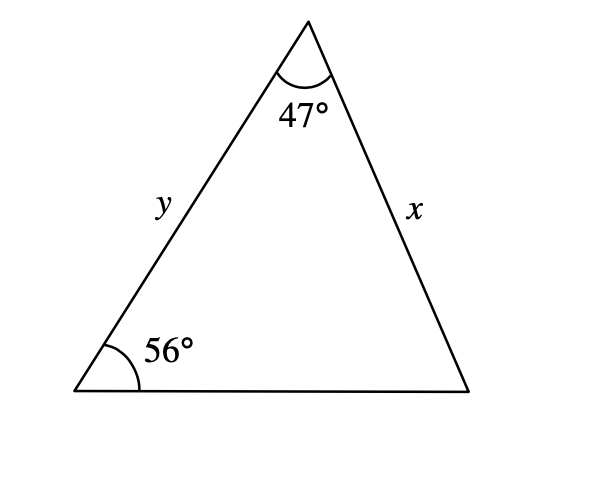
\includegraphics[width = 0.7\textwidth]{SPFigure2.38.png}	
	\end{figure}
	\begin{enumerate}
		\item[A.] $\dfrac{x\sin{77^\circ}}{\sin{56^\circ}}$.
		\item[B.] $\dfrac{x\sin{47^\circ}}{\sin{56^\circ}}$.
		\item[C.] $\dfrac{x\sin{56^\circ}}{\sin{77^\circ}}$.
		\item[D.] $\dfrac{x\sin{77^\circ}}{\sin{47^\circ}}$.
	\end{enumerate}
	
	\item \textbf{HKDSE MATH Core Sample Paper II Q39}\\
	Peter invests \$ $P$ at the beginning of each month in a year at an interest rate of 6\% per annum, compounded monthly. If he gets \$10 000 at the end of the year, find $P$ correct to the 2 decimal places.
	\begin{enumerate}
		\item[A.] 806.63
		\item[B.] 829.19
		\item[C.] 833.33
		\item[D.] 882.18
	\end{enumerate}
	
	\item \textbf{HKDSE MATH Core Sample Paper II Q40}\\
	The figure shows a cuboid $ABCDEFGH$. If the angle between the triangle $ACE$ and the plane $ABCD$ is $\theta$, then $\tan{\theta} = $
	\begin{figure}[H]
		\centering
		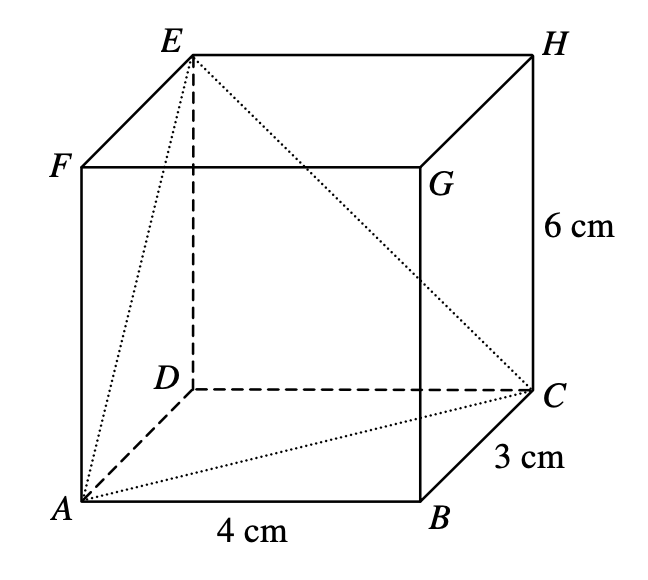
\includegraphics[width = 0.7\textwidth]{SPFigure2.40.png}	
	\end{figure}
	\begin{enumerate}
		\item[A.] 2.
		\item[B.] $\dfrac{3}{2}$.
		\item[C.] $\dfrac{5}{2}$.
		\item[D.] $\dfrac{12}{5}$.
	\end{enumerate}
	
	\item \textbf{HKDSE MATH Core Sample Paper II Q41}\\
	In the figure, $A$, $B$ and $C$ are points lying on the circle. $TA$ is the tangent to the circle at $A$. The straight line $CBT$ is perpendicular to $TA$. If $BC = 6$ cm, find the radius of the circle correct to the nearest 0.1 cm.
	\begin{figure}[H]
		\centering
		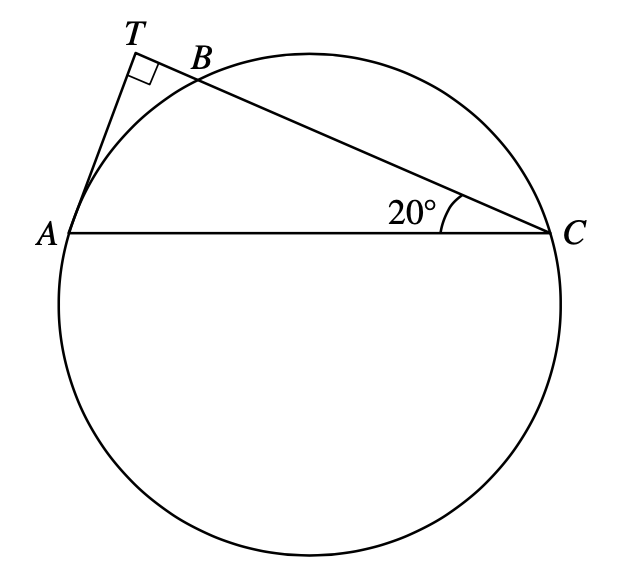
\includegraphics[width = 0.7\textwidth]{SPFigure2.41.png}	
	\end{figure}
	\begin{enumerate}
		\item[A.] 3.2 cm
		\item[B.] 3.9 cm
		\item[C.] 4.2 cm
		\item[D.] 4.7 cm
	\end{enumerate}
	
	\item \textbf{HKDSE MATH Core Sample Paper II Q42}\\
	Let $a$ be a constant and $-90^\circ < b < 90^\circ$. If the figure shows the graph of $y = a\cos{(x^\circ + b)}$, then 
	\begin{figure}[H]
		\centering
		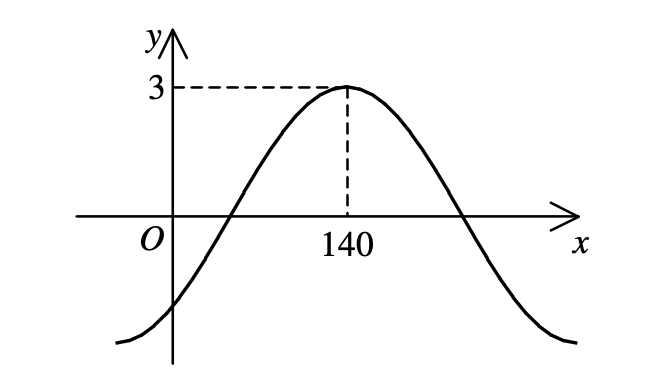
\includegraphics[width = 0.7\textwidth]{SPFigure2.42.png}	
	\end{figure}
	\begin{enumerate}
		\item[A.] $a = -3$ and $b = -40^\circ$.
		\item[B.] $a = -3$ and $b = 40^\circ$.
		\item[C.] $a = 3$ and $b = -40^\circ$.
		\item[D.] $a = 3$ and $b = 40^\circ$.
	\end{enumerate}
	
	\item \textbf{HKDSE MATH Core Sample Paper II Q43}\\
	Bag $A$ contains 2 red balls, 3 green balls and 4 white balls while bag $B$ contains 2 red balls, 3 green balls and 4 yellow balls. If one ball is drawn randomly from each bag, then the probability that the two balls drawn are of different colours is
	\begin{enumerate}
		\item[A.] $\dfrac{13}{81}$.
		\item[B.] $\dfrac{29}{81}$.
		\item[C.] $\dfrac{52}{81}$.
		\item[D.] $\dfrac{68}{81}$.
	\end{enumerate}
	
	\item \textbf{HKDSE MATH Core Sample Paper II Q44}\\
	If 2 girls and 5 boys randomly form a queue, find the probability that the two girls are next to each other in the queue.
	\begin{enumerate}
		\item[A.] $\dfrac{1}{7}$
		\item[B.] $\dfrac{2}{7}$
		\item[C.] $\dfrac{6}{7}$
		\item[D.] $\dfrac{1}{21}$
	\end{enumerate}
	
	\item \textbf{HKDSE MATH Core Sample Paper II Q45}\\
	A set of numbers has a mode of 32, an inter-quartile range of 27 and a variance of 25. If 3 is added to each number of the set and each resulting number is then doubled to form a new set of numbers, find the mode, the inter-quartile range and the variance of the new set of numbers.
	$\begin{matrix}
	&\text{Mode}&\text{Inter-quartile range}&\text{Variance}\\
	\text{A.}&64&60&50\\
	\text{B.}&70&60&100\\
	\text{C.}&70&54&50\\
	\text{D.}&70&54&100\\
	\end{matrix}$

\end{enumerate}
\end{document}

